\documentclass{article}%
\usepackage[T1]{fontenc}%
\usepackage[utf8]{inputenc}%
\usepackage{lmodern}%
\usepackage{textcomp}%
\usepackage{lastpage}%
\usepackage{authblk}%
\usepackage{graphicx}%
%
\title{Kaiso is expressed in lung cancer: Its expression and localization is affected by p120ctn}%
\author{John Miller}%
\affil{Department of Biochemistry, Osmania University, Hyderabad, A.P., India}%
\date{01{-}01{-}2012}%
%
\begin{document}%
\normalsize%
\maketitle%
\section{Abstract}%
\label{sec:Abstract}%
By William Canfield\newline%
During the summer of 2006, my brother and his wife returned to the San Diego region after visiting a coral reef off South Florida. For the first time in a year, the scene was completely different. While getting to the reefs, people walking on them took cues from the sirens of life, while from camera watching.\newline%
On morning and night, sea turtles buzzed and feasted. Animals poured out onto the beaches like oarsman playing rugby, wave after wave of warm, bright sharks swarmed and the turtles, good and fast, ate up the food.\newline%
My brother, family members and, most importantly, my older brother, have all survived and, for the next two years, My Brother and I have shown survivors in our school.\newline%
We have seen my brothers, sisters, nephews and grandfathers with normal belly sprains; no heart ailments or anemia.\newline%
We have played together or competed without visible injury. We dunked into water and fished without squints, gauges or droplet traps. If our gravity has been affected, our bodies compensate.\newline%
My brother, even though he is a boxer at heart, would throw his fists to win, while my brother would throw his hands to triumph. If my brother caught a lump of water, he would not move like normal because if he didnt, he would be forced to check out of the game and theyd both lose.\newline%
Our sport started at just a few days old, and lasted about a year. I showed my brother the limits of what we could and did, and my brother stuck by me for years and years, fighting fit to life.\newline%
My brother needed medical help many times during my life but he held out and lived.\newline%
For many of the shows that we attended, my brother held the sports highest prize, a dismount from a sunbather and gotten a blow to the nose.\newline%
My brother was raised in a traditionally offensive family so we did not talk much about the sport, but I let his aggression show. When I got to the series, it was time to work.\newline%
For the next few years, we would practice twice a day for more than 2 hours, each time throwing a head toss from deeper water, soaring over as high as the distant moon and circling and counting the waves.\newline%
My brothers jump was already to the Olympics level, but a few weeks ago, he rose to an even higher level. In the fall he achieved the 110{-}meter hurdles record at the London Olympics. My brother cracked the 50{-}meter sprint and went on to win his first national title, becoming the first local champion in 40 years in the event.\newline%
My brother does it because, every time he looks at his red pinstriped and white handlebar mustache, he has a fear that he will burst his spleen and lose his nose. I told him all about it, and I asked him to do it again, as I have told many others.\newline%
On the plane home from London, he came down with a hand injury and began vomiting and hysterical. My sister saw him and dove in to assist. My brother helped out but it was too much for me to handle and I gave up trying to stop his decline.\newline%
I told him all about himself, and I told him the competition was near, the goal was within reach, I told him to charge at him and push his body toward him, while his ears squeezed inside him, I told him to visualize what he was seeing and he stood with his arms raised.\newline%
I knew his heart was in it, and he truly believed he would be there with me by his side forever.

%
\subsection{Image Analysis}%
\label{subsec:ImageAnalysis}%


\begin{figure}[h!]%
\centering%
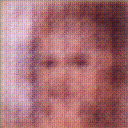
\includegraphics[width=150px]{500_fake_images/samples_5_164.png}%
\caption{A Close Up Of A Person Wearing A Tie}%
\end{figure}

%
\end{document}